\documentclass{article}
\usepackage[utf8]{inputenc}
\usepackage{natbib}
\usepackage{graphicx}
\usepackage{vmargin}
\usepackage{hyperref}
\usepackage{booktabs}
\usepackage{multirow}
\usepackage{siunitx}
\setpapersize{A4}
\setlength{\parskip}{\baselineskip}%
\setlength{\parindent}{0pt}%

\title{Entregable WEKA}
\author{Laura Rodríguez Navas \\ rodrigueznavas@posgrado.uimp.es}
\date{Marzo 2020}

\begin{document}

\maketitle

\section*{Preparación de datos}

Consideramos la base de datos Prostate definida sobre 12600 variables predictivas (todas numéricas) y una variable clase binaria \{tumor, normal\}. Está formada por 136 registros y en ella no existen valores desconocidos. Pero está ordenada en función de la variable clase \{Tumor, Normal\}. Como consecuencia, tenemos que aleatorizar la base de datos. Para ello se aplica un filtro a nivel de registro, concretamente de tipo no supervisado llamado Ramdomize. Usamos la semilla que viene por defecto (42).

A continuación, dividimos la base de datos en un conjunto de entrenamiento, con dos tercios de los registros, y un conjunto de test con un tercio de los registros. Para ello se aplica un filtro a nivel de registro y no supervisado llamado RemoveFolds. Como resultado hemos creado un conjunto de entrenamiento con 90 registros.

Observamos que la distribución de la variable clase en el conjunto de entrenamiento no es uniforme.

\begin{center}
	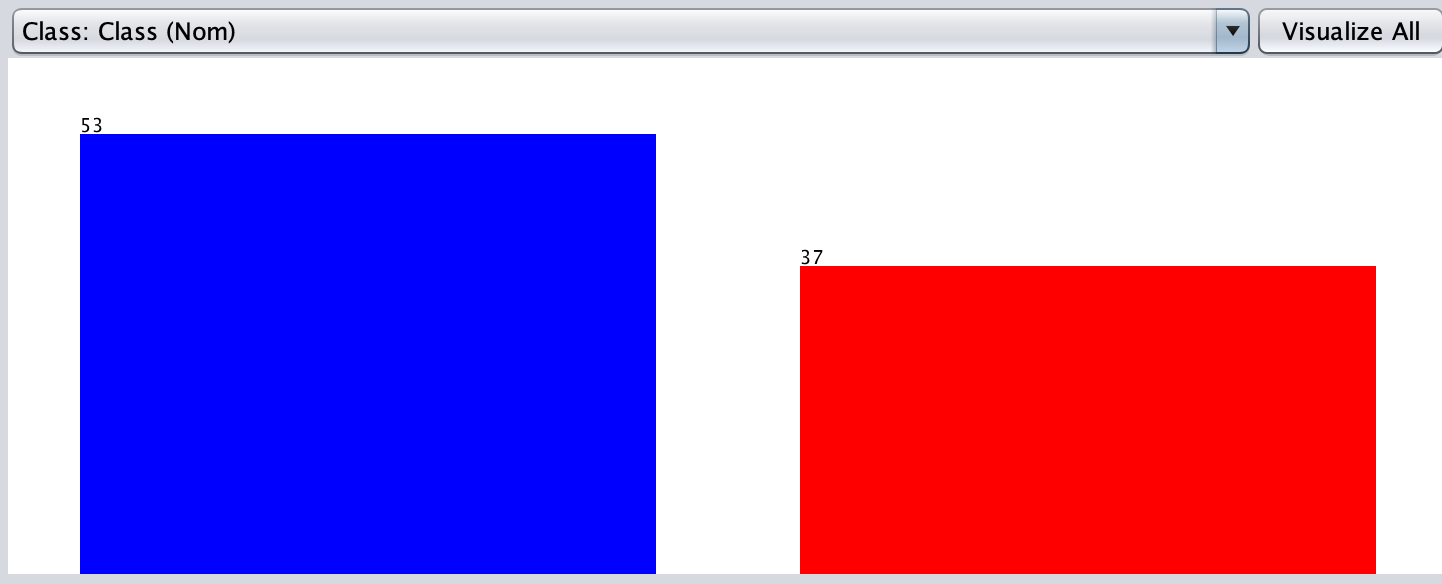
\includegraphics[scale=0.3]{distribucion_norm.png}
\end{center}

\section*{Clasificación}

Se usan los clasificadores NaiveBayes y J48 (C4.5) en una validación cruzada de 5 carpetas (5cv) sobre el conjunto de entrenamiento de la base de datos.

Se han considerado dos parámetros de rendimiento para la evaluación de los resultados. Los siguientes parámetros son examinados antes de la discretización y la selección de variables: Accuracy y Error Rate. 

\begin{center}
	\begin{tabular}{ |c|c|c| } 
		\hline
		Clasificador & Acc. en \% & ERR en \% \\
		\hline
		NaiveBayes & 52.2222 & 47.7778 \\ 
		J48 & 82.2222 & 17.7778 \\ 
		\hline
	\end{tabular}
\end{center}

Como podemos observar el clasificador J48 es mucho mejor que NaiveBayes.

\section*{Mejoras}
\subsection*{Discretización}

Primero utilizamos un método supervisado a nivel de atributo. Como resultado, los parámetros Accuracy y Error Rate resultantes de la ejecución de los clasificadores después de la discretización son:

\begin{center}
	\begin{tabular}{cSSSSS}
		\toprule
		\multirow{2}{*}{Clasificador} &
		\multicolumn{2}{c}{Antes Disc.} &
		\multicolumn{2}{c}{Después Disc.} \\
		& {Acc in \%} & {ERR in \%} & {Acc in \%} & {ERR in \%} \\
		\midrule
		NaivesBayes & 52.2222 & 47.7778 & 82.2222 & 17.7778 \\
		J48 & 82.2222 & 17.7778 & 87.7778 & 12.2222 \\
		\bottomrule
	\end{tabular}
\end{center}

Después, utilizamos dos métodos no supervisados a nivel de atributo.

\begin{center}
	\begin{itemize}
		\item Intervalos de igual amplitud \\
		\begin{tabular}{ |c|c|c| } 
			\hline
			\# of bins & Acc. en \% & ERR en \% \\
			\hline
			2 & 52.2222 & 47.7778 \\ 
			4 & 82.2222 & 17.7778 \\ 
			5 & 52.2222 & 47.7778 \\ 
			10 & 82.2222 & 17.7778 \\ 
			\hline
		\end{tabular}
		\item Intervalos de igual frecuencia \\
		\begin{tabular}{ |c|c|c| } 
			\hline
			\# of bins & Acc. en \% & ERR en \% \\
			\hline
			2 & 52.2222 & 47.7778 \\ 
			4 & 82.2222 & 17.7778 \\ 
			5 & 52.2222 & 47.7778 \\ 
			10 & 82.2222 & 17.7778 \\ 
			\hline
		\end{tabular}
	\end{itemize}
\end{center}

Finalmente,

\begin{center}
	\begin{tabular}{cSSSSS}
		\toprule
		\multirow{2}{*}{Clasificador} &
		\multicolumn{2}{c}{Antes Disc.} &
		\multicolumn{2}{c}{Después Disc.} \\
		& {Acc in \%} & {ERR in \%} & {Acc in \%} & {ERR in \%} \\
		\midrule
		NaivesBayes & 52.2222 & 47.7778 & 55.1471 & 44.8529 \\
		J48 & 82.2222 & 17.7778 & 74.2647 & 25.7353 \\
		\bottomrule
	\end{tabular}
\end{center}

\subsection*{Selección de variables}

\end{document}
